\chapter{Mask R-CNN}
\noindent

\section{The problem with Faster R-CNN}
\label{section:problemofFasterRCNN}
\noindent

	Until now, we know how Faster R-CNN extract feature maps by passing the image through lots of convolutional layer. However, while down sampling the image, we also scaled down the RoIs inside the image with a specific factor and round the offset of their bounding boxes. As a result, we create a new bounding box for the object inside which cause missing information and reduce performance of our system.
	
	An example \ref{fig:quantization_problem}, it illustrates when we feed 512x512 image to VGG16 and cause quantization on bounding box offset. The blue part is the missing piece data and the one green is a new data created by quantization.
	
	\begin{figure}[H]
		\centering
		{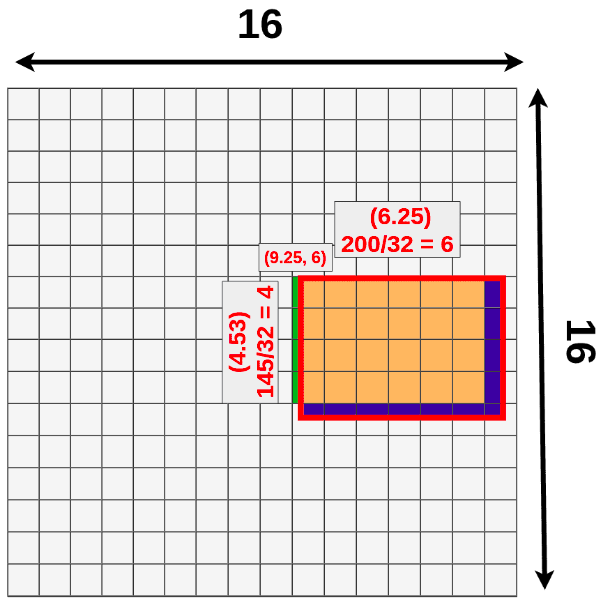
\includegraphics[width=0.4\textwidth]{./hinhanh/chap5/problem.png}}
		\caption{Example of quantization problem causing missing information.}
		\label{fig:quantization_problem}
	\end{figure}
	
	As mention before in \ref{subsection:roi_pool}, RoI pooling operation will quantize floating number of RoI offset to a discrete offset. Then this quantized RoI is subdivided into spatial bins which are then aggregated (usually by max pooling) \cite{fasterrcnn}. And once again, we lose vector information. We can look at \ref{fig:quantization_problem} for more details.

\section{An extended solving the problem - Mask R-CNN}
\label{section:maskrcnn}
\noindent

	In 2017, a group of Facebook AI researchers - Kaiming He at el presented a new system which is influenced by Faster R-CNN called Mask R-CNN. This system, gennerally, is an extend of Faster R-CNN with a new branch for segmentation generating an object mask. Unlike others system which are complex multiple-stage cascade that predicts segment proposals from bounding-box proposals, followed by classification. Mask R-CNN allows three branches (including the existing branch for classification and bounding box regression, and a branch for predicting segmentation masks on RoI) to run in parallel which enhance the processing speed.	
	
	\begin{figure}[H]
		\centering
		{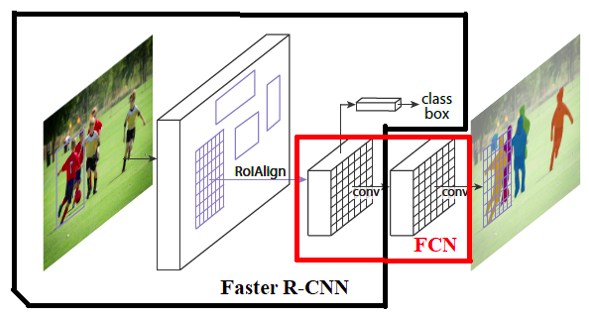
\includegraphics[width=0.6\textwidth]{./hinhanh/chap5/mask_rcnn.png}}
		\caption{Mask R-CNN architecture including Faster R-CNN and FCN}
		\label{fig:maskrcnn}
	\end{figure}
	
	As \ref{fig:maskrcnn} shows that Mask R-CNN is constructed by Faster R-CNN and a small fully convolution neural network. Because it is a stack of convolutional layer, the mask branch only consumes a small computational resource enabling the system to run extremely fast in testing phrase just like Faster R-CNN speed (~0.2s/image). 
	
	It is noticeable that Mask R-CNN’s authors solved the problem of RoI Pooling quantization by proposing a brand-new alternative technique called RoI Align which completely secure spatial locations of bounding box and information inside it. According to the paper, this minor change can affect the result accuracy up to 50\%.
	
\subsection{Multi-task loss}
\label{subsection:multitaskloss}
\noindent
	
	Inherit the spirit of Faster R-CNN, Mask R-CNN also has two stage procedure, with RPN is the first stage that generates proposals. In the next stage, in parallel with the original branch of Fast R-CNN, there is a mask generation branch that outputs a binary mask for each RoI. Therefore, a new loss function was proposed and defined as $ \L = L_{cls} + L_{box} + L_{mask}\ $. The classification and regression loss ($ \ L_{cls}, L_{box} \ $) are the same as those defined in \cite{fastrcnn}. 
	
	The mask loss, according to the authors, was defined as the average binary cross entropy loss (per-pixel sigmoid and binary loss) enabling the system to generate masks for each class without causing competition among them. As a result, lots of masks will be generated but only the ground truth masks of class k in the corresponding RoIs are considered while calculating the mask loss (masks on another classes are not contribute to mask loss of class k). And by taking advantage of the classifier branch, the predicted class will be used to choose the output mask. This strategy decouples the mask and class prediction and outputs good instance segmentation results. Therefore, Mask R-CNN’s strategy is different from most techniques at that time (in semantic segmentation problems) when adopting a per-pixel multinomial logistic loss and validate with the standard metric of mean pixel intersection over union (IoU), with the mean taken over all classes - softmax (competition between classes), including background \cite{maskrcnn}.
	
	\[ L_{mask} = -\frac{1}{m^2} \sum_{1 \leqslant i, j \leqslant m} [ y_{ij}log\hat{y}^k_{ij} + (1-y_{ij})log(1-\hat{y}^k_{ij}) ] \]
	
\subsection{Mask representation}
\label{subsection:mask_representation}
\noindent
	
	Different from label and offset branch that collapse the feature map into a fixed-vector by using FC layer. Mask branch generates a mash that represents the object area in the input image. To be more specific, it encodes object's spatial information to a binary map that separates the object from the background. To achieve this goal, naturally, Mask R-CNN adopts a FCN to extract pixel-to-pixel information by taking advantage of convolution operations.
	
	So instead of adopting a FC layer to classify each pixel and generate mask from it, the FCN uses fewer parameters, and is more efficient than the FC layer. However, to preserve mask generating's efficiency, RoI must be extracted without losing minimum information so that the spacial structure correspondence to original input image will be maintain accurately. Therefore, RoI align layer plays a crucial role in Mask RCNN \cite{maskrcnn}.
	
\subsection{RoI align}
\label{subsection:roialign}
\noindent
	
	As mentioned before in \ref{subsection:roi_pool} and \ref{section:problemofFasterRCNN}, RoI pooling's quantization causes missing information two times in it process. Firstly, a quantization operations is executed to map the generated RoI's coordinates (x, y indexes) from floating values to integer ones. Secondly, this quantized RoI is then sub-divided into small boxes whose size are rounded up. As a result, these quantization operations lead us to the problem of misalignment between the RoI and the extracted feature map. Even though, it does not affect the classification or detection task due to the robustness on small adjustment, it is extremely sensitive on the pixel predicting of the segmentation task and impact directly to the model performance.
	
	To address the problem, Kaiming He and his partners proposed a method called RoI align that erase the harassment of quantization from RoI pool technique. The change is minor but it works significantly effective on segmentation task. By taking advantage of bi-linear interpolation, the whole quantization issue is solved. Similar to RoI pool method, the RoI is divided into pre-fixed number of smaller regions. Within each smaller regions, 4 points are sampled. To be more specific, the calculation does not fall on a specific pixel, and the nearest pixel is used to perform bilinear interpolation on this \textit{virtual pixel} to obtain the pixel value and then max or average operation is executed to get the final result \cite{maskrcnn}.




